\subsection{Resolution and Representation Sensitivity}
A uniform 20,000-wallet sample from the complete annual feature file was used for a common exploratory sweep over $k=2$--10. Each candidate was fitted using mini-batch k-means with ten initializations and seeds 492--496. Silhouette used the same 2,000-row evaluation subset for each fit. Reported standard deviations describe variation across fits on this diagnostic sample, not population confidence intervals. The original annual scaler was retained for this sensitivity experiment.
\begin{table}[t]\centering\caption{Common exploratory sample sweep.}\label{tab:review_sweep}\small
\begin{tabular}{crr}\toprule $k$ & Silhouette (mean $\pm$ SD) & Mean DB \\\midrule
2 & $0.208 \pm 0.027$ & 1.899 \\
3 & $0.184 \pm 0.054$ & 1.795 \\
4 & $0.166 \pm 0.007$ & 1.666 \\
5 & $0.170 \pm 0.002$ & 1.639 \\
6 & $0.145 \pm 0.024$ & 1.746 \\
7 & $0.158 \pm 0.016$ & 1.725 \\
8 & $0.144 \pm 0.021$ & 1.731 \\
9 & $0.139 \pm 0.011$ & 1.690 \\
10 & $0.141 \pm 0.011$ & 1.707 \\
\bottomrule\end{tabular}\end{table}
The largest mean silhouette occurs at $k=2$, whereas the smallest mean Davies--Bouldin index occurs at $k=5$. The sweep therefore does not establish $k=4$--6 as the only admissible range. We retain it as an exploratory neighbouring-resolution comparison.
Seed-pair agreement, repeated 80\% subsampling, a disjoint activity/value/other feature-group weighting check, full k-means, and a diagonal-covariance Gaussian mixture were evaluated on the same diagnostic sample. These comparisons test sensitivity rather than establish that one algorithm is correct.
\begin{table}[t]\centering\caption{Sample representation sensitivity: ARI against the reference sample fit.}\small
\begin{tabular}{crrr}\toprule $k$ & Count only & Equal group weight & Full k-means \\\midrule
4 & 0.308 & 0.465 & 0.697 \\
5 & 0.252 & 0.422 & 0.864 \\
6 & 0.172 & 0.449 & 0.376 \\
\bottomrule\end{tabular}\end{table}
Full-cohort overlap compares all 2,443,868 annual EOAs. The ARIs for K4/K5, K4/K6, and K5/K6 are respectively 0.626, 0.517, 0.642. For example, K4 role 0 distributes 37.7\% and 62.2\% of its wallets into K5 roles 3 and 4; K5 role 1 distributes 53.8\% and 43.5\% into K6 roles 0 and 5. Cluster numbers are local identifiers and the partitions are not assumed to form a hierarchy.
\begin{figure}[t]\centering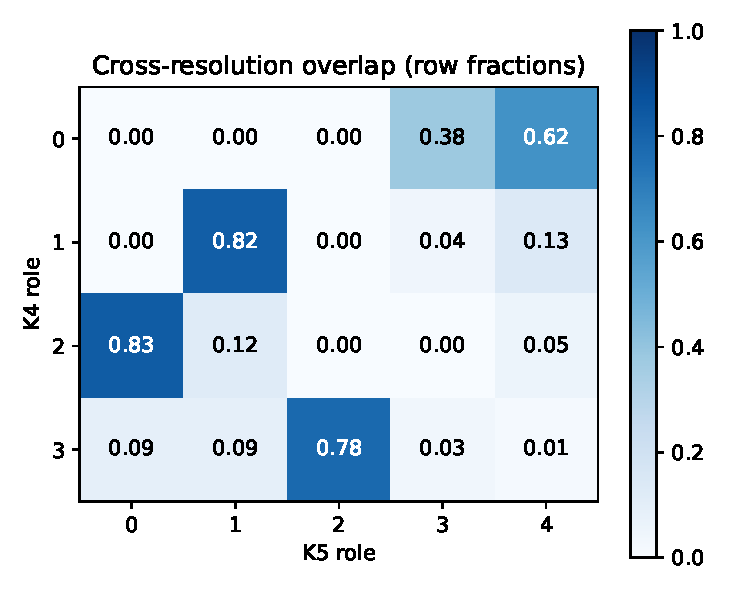
\includegraphics[width=\columnwidth]{figures/review_k4_k5_overlap.pdf}\caption{Full-cohort K4/K5 overlap. Each row sums to one; identifiers are local to each partition.}\label{fig:review_overlap}\end{figure}
\begin{table}[t]\centering\caption{Comparable full-cohort feature holdouts: ARI.}\small
\begin{tabular}{lrrr}\toprule Removed family & K4 & K5 & K6 \\\midrule
Activity & 0.473 & 0.370 & 0.527 \\
Value flow & 0.266 & 0.239 & 0.302 \\
Directionality & 0.615 & 0.462 & 0.422 \\
Volatility & 0.507 & 0.503 & 0.607 \\
Persistence & 0.497 & 0.413 & 0.461 \\
\bottomrule\end{tabular}\end{table}
\subsection{Corrected Monthly Count-State Evaluation}
To avoid annual/monthly window mismatch and pooled token denominations, this separate analysis uses six monthly count features: transactions per calendar day, active-day fraction, transactions per active day, calendar-day count coefficient of variation, peak-day transaction share, and active-span fraction. The intensity and coefficient-of-variation features receive log1p transforms. A common RobustScaler and K4/K5/K6 prototypes are fitted on up to 20,000 active wallet-months from each of January--June (seed 492; ten initializations), then frozen. Missing wallet-months remain missing, and monthly state numbers are separate from annual role identifiers.
Evaluation uses July--December only. Persistence is conditional on activity in adjacent months. Return tests use first-step switchers active in each of three consecutive months and shuffle final states within middle-state strata, with 999 permutations. Holm correction covers all twelve held-out return tests across the three resolutions. The annual EOA cohort is retrospectively defined; this is a later-period within-cohort test, not prospective validation on unseen users.
\begin{table}[t]\centering\caption{Frozen count-state evaluation, July--December.}\label{tab:corrected_temporal}\small
\begin{tabular}{crrrr}\toprule $k$ & Persistence & Chance & $\kappa$ & Return (null) \\\midrule
4 & 55.5\% & 40.7\% & 0.250 & 40.8\% (37.0\%) \\
5 & 46.6\% & 31.0\% & 0.226 & 33.6\% (27.8\%) \\
6 & 37.0\% & 23.4\% & 0.178 & 27.9\% (22.8\%) \\
\bottomrule\end{tabular}\end{table}
All twelve held-out return tests have raw $p=0.001$ and joint Holm-adjusted $p=0.012$, the resolution supported by 999 null draws with no exceedances. Conditional next-state entropy reductions are 12.1\%, 10.2\%, and 9.4\% for K4, K5, and K6. These results support temporal organization across the three count-state resolutions. They do not establish the correctness of the original value-based annual labels or eliminate stable wallet heterogeneity.
\subsection{Count-Preserving Timing Surrogates}
A uniform sample of 500 annual EOAs was represented by all 365 daily transaction counts. Each surrogate permutes the daily counts within each wallet, preserving its count distribution, total activity, and active-day count. All 500 observed signals had positive non-DC power. Across 999 surrogate replicates, three upper-tail tests compare sample-mean low-frequency share, peak-power share, and negative spectral entropy. Holm correction covers these three summaries.
Observed low-frequency share was 0.1055 versus a null mean of 0.0330; peak-power share was 0.0449 versus 0.0264; spectral entropy was 6.815 versus 6.969 bits. All three adjusted $p$-values were 0.003. This supports timing organization beyond the preserved daily-count distribution in this wallet sample; it does not establish recurring annual cycles or validate a specific annual partition.
\subsection{Held-Out Participation Prediction}
We test whether the corrected monthly states summarize subsequent participation. Among wallets active in the current month, the target is activity in the following month. Predictions are trained on January--May pairs (up to 50,000 active wallets per month) and evaluated on all active wallets in July--November pairs. State-only predictors use smoothed training-state participation rates. Baselines are the training prevalence and logistic regression on log-transformed transaction intensity and active-day fraction. Wallets can recur between periods; this tests later time periods within the retrospective cohort, not unseen people.
\begin{table}[t]\centering\caption{Later-period prediction. Losses are weighted by evaluation pair size; lower is better.}\small
\begin{tabular}{lrr}\toprule Predictor & Brier loss & Log loss \\\midrule
Activity logistic & 0.2092 & 0.6044 \\
Constant & 0.2237 & 0.6396 \\
K4 states & 0.2125 & 0.6132 \\
K5 states & 0.2112 & 0.6099 \\
K6 states & 0.2108 & 0.6088 \\
\bottomrule\end{tabular}\end{table}
State-only predictors improve on constant prevalence, but the simple activity logistic baseline has lower Brier and log loss in every evaluation month than any state-only predictor. The task therefore does not demonstrate incremental predictive value of the monthly segmentation over direct activity features. Interpretability and compression require their own evaluation; they cannot be inferred from statistically significant temporal persistence.
\subsection{Activity-Conditioned Network Evaluation}
A separate network analysis streams all twelve monthly raw files for coverage and in/out transfer-event counts. Each month retains a uniform priority sample of 50,000 non-self transfer events with two labelled EOA endpoints. Wallet labels are shuffled either unrestricted among participating EOAs or within joint logarithmic in/out event-count bins fitted using the complete retained monthly graph. The bins condition on activity approximately; they are not exact unique-neighbour degree matching. The full-mixing statistic is mutual information between sender and recipient role, which can detect complementary cross-role organization even when same-role concentration is weak.
For each resolution, null, and metric, 999 Monte Carlo draws produce upper-tail tests with Holm correction over twelve months. This defines separate testing families, not a single joint rejection across every analysis. Marginal draws on sampled endpoints use a multivariate hypergeometric distribution equivalent to restricting full within-stratum label permutations to those endpoints. No independence-calibrated combination across months is used.
The retained two-labelled-EOA non-self transfers constitute 15.1\% of all raw transfers (monthly range 13.2--18.7\%). Exclusions include contracts and addresses outside the labelled cohort; these causes are not separated by this coverage statistic. The tests describe this retained subgraph and its event sample.
\begin{table}[t]\centering\caption{Monthly rejections after Holm correction within each candidate/null/metric family. Full mixing uses role mutual information.}\small
\begin{tabular}{llrrr}\toprule Null & Metric & K4 & K5 & K6 \\\midrule
Unrestricted & Same role & 12/12 & 1/12 & 11/12 \\
Unrestricted & Full mixing & 12/12 & 12/12 & 12/12 \\
Activity bins & Same role & 2/12 & 12/12 & 12/12 \\
Activity bins & Full mixing & 12/12 & 12/12 & 12/12 \\
\bottomrule\end{tabular}\end{table}
Conditioned effects and full-mixing tests address different questions from unrestricted homophily. Significant full mixing is an association between endpoint labels under this null, not evidence of identity, causality, or uniformly positive same-role preference.
